\documentclass[border=3pt,tikz]{standalone}
% Shared look for every TikZ figure in these notes.
% Included by each standalone figure file; also keeps the figures consistent
% with the colours used in the PDF and on the website.

\usepackage{tikz}
\usepackage{pgfplots}
\pgfplotsset{compat=1.18}
\usetikzlibrary{arrows.meta, decorations.markings, decorations.pathmorphing,
                patterns, calc, positioning}
\usepackage{amsmath}

% Series colours are the three validated categorical slots also used by the
% interactive widgets, so a path drawn in the printed notes and the same path on
% the website are the same colour. They clear the colour-vision-deficiency and
% contrast checks as a set; every path is direct-labelled as well, so colour is
% never the only thing carrying identity.
\definecolor{duPurple}{HTML}{68246D}
\definecolor{duBlue}{HTML}{2A78D6}
\definecolor{duRed}{HTML}{EB6834}
\definecolor{duGreen}{HTML}{1BAF7A}
\definecolor{duGrey}{HTML}{6B6B6B}

\tikzset{
  axisline/.style   = {-{Stealth[length=3mm]}, line width=0.7pt, black},
  path1/.style      = {duBlue,   line width=1.1pt},
  path2/.style      = {duRed,    line width=1.1pt},
  path3/.style      = {duGreen,  line width=1.1pt},
  statedot/.style   = {circle, fill=black, inner sep=1.4pt},
  arrowhead/.style  = {decoration={markings,
                        mark=at position #1 with {\arrow{Stealth[length=2.6mm]}}},
                       postaction={decorate}},
  lbl/.style        = {font=\small},
  slbl/.style       = {font=\footnotesize, duGrey},
  workfill/.style   = {duPurple, opacity=0.16},
}

\begin{document}
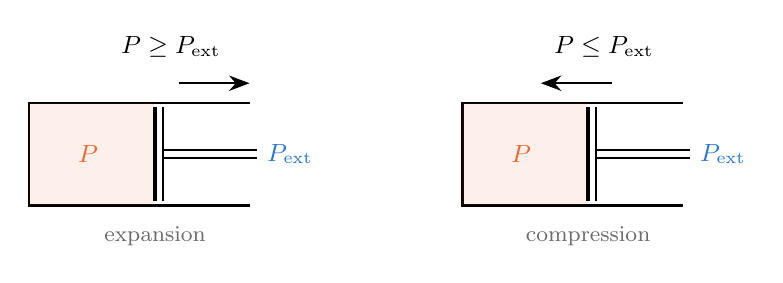
\begin{tikzpicture}
\newcommand{\cyl}[4]{% x-shift, title, relation, arrow direction (+1 / -1)
  \begin{scope}[shift={(#1,0)}]
    \draw[line width=1pt] (2.8,1.3) -- (0,1.3) -- (0,0) -- (2.8,0);
    \fill[duRed, opacity=0.10] (0,0) rectangle (1.6,1.3);
    \draw[line width=1.6pt] (1.6,0.05) -- (1.6,1.25);
    \draw[line width=0.9pt] (1.7,0.6) -- (2.9,0.6);
    \draw[line width=0.9pt] (1.7,0.7) -- (2.9,0.7);
    \draw[line width=0.9pt] (1.7,0.05) -- (1.7,1.25);
    \node[lbl, duRed] at (0.75,0.65) {$P$};
    \node[lbl, duBlue, right] at (2.9,0.65) {$P_\text{ext}$};
    \draw[-{Stealth[length=2.6mm]}, line width=0.8pt] (1.9,1.55) -- ++(#4*0.9,0);
    \node[lbl, above] at (1.8,1.75) {#3};
    \node[slbl, below] at (1.6,-0.15) {#2};
  \end{scope}}
\cyl{0}{expansion}{$P \ge P_\text{ext}$}{1}
\cyl{5.5}{compression}{$P \le P_\text{ext}$}{-1}
\end{tikzpicture}
\end{document}
